\begin{enumerate}[label=\thesubsection.\arabic*.,ref=\thesubsection.\theenumi]
\numberwithin{equation}{enumi}
\item Find the peak Overshoot due to a unit step input for the following second order control system.
\begin{align}
    G(S) = \frac{100}{s^2 + 10s +100}    
\end{align}

The transfer function for the second order control system is:
\begin{equation}
    \dfrac{C(s)}{R(s)}= \dfrac{\omega_n^2}{s^2 + 2\zeta\omega_ns + \omega_n^2}
\end{equation}
To calculate the unit step response,
\\
Put $r(t) = 1$ or $R(s) = \dfrac{1}{s}$
\\
On Simplifying, 
\begin{align}
    C(s) = \frac{1}{s}-\frac{s+\zeta\omega_n}{(s + \zeta\omega_n)^2 + \omega_d^2} - \frac{\zeta\omega_n}{\omega_d}.\frac{\omega_d}{(s + \zeta\omega_n)^2 + \omega_d^2}  
\end{align}
where, $\omega_d=\omega_n\sqrt{1-\zeta^2}$
\\In time domain, c(t) = $\mathcal{L}^{-1}{C(s)}$. Using this:
\begin{align}
    c(t) = 1 - e^-\zeta\omega_nt(cos\omega_dt+\dfrac{\zeta}{\sqrt{1-\zeta^2}}.sin\omega_dt)
    \label{eq:eebtech11045_ct}
\end{align}

 \textbf{Peak Overshoot:}
 Peak Overshoot is the difference between the magnitude of the highest peak of time response and magnitude in its steady state. Peak Overshoot is expressed in term of percentage of steady-state value of the response.
\begin{align}
\implies M_p = \dfrac{c(t_p) - c(\infty)}{c(\infty)} * 100 \%
\end{align}
To find Peak Overshoot:
\\
\\
c(t) is max where $\dfrac{dc(\emph{t})}{d(\emph{t})}$ = 0
\\
Applying this condition on \eqref{eq:eebtech11045_ct}:
\begin{align}
    \implies t = \frac{\pi}{\omega_n\sqrt{1-\zeta^2}}
\end{align}
\\Substituting this value of t in \eqref{eq:eebtech11045_ct}:
\begin{align}
    M_p (PeakOvershoot) = e^{\dfrac{-\zeta\pi}{\sqrt{1-\zeta^2}}}
    \label{eq:ee18btech11045_Mp}
\end{align}
\\
For the given Equation : G(S) = $\dfrac{100}{s^2 + 10s +100}$
$\zeta = 0.5$
\\
Substituting $\zeta = 0.5$ in \eqref{eq:ee18btech11045_Mp}, we get:
\\
Peak Overshoot = 0.163
\\
\\
\textbf{Plotting c(t)}
\begin{figure}[!h]
    \centering
    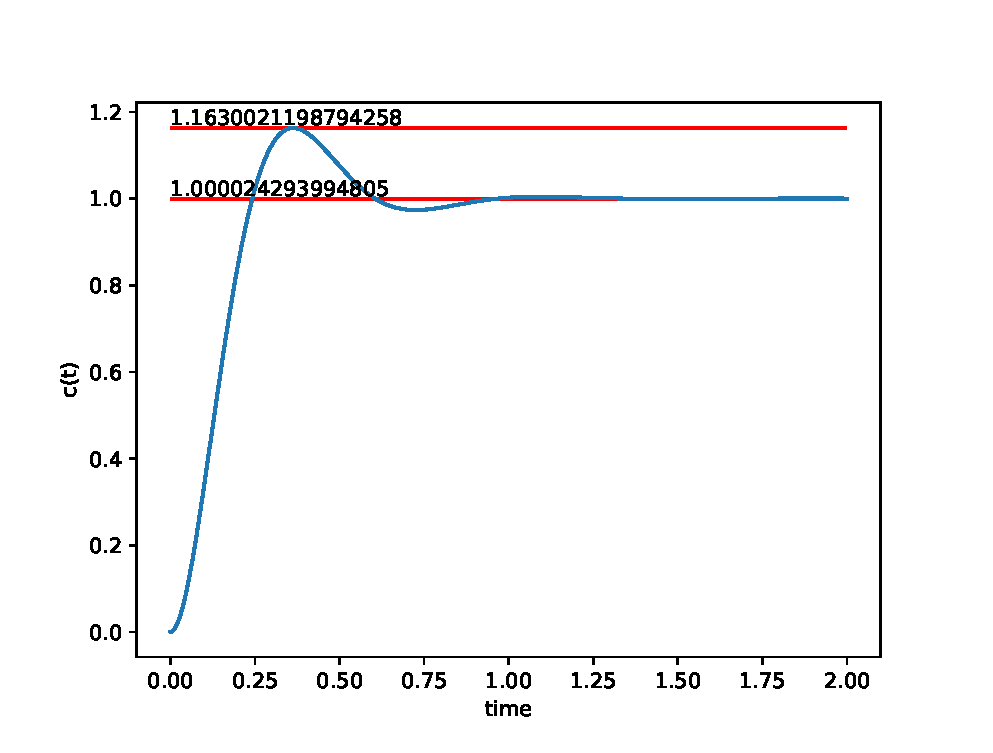
\includegraphics[width=\columnwidth]{./figs/ee18btech11045/ee18btech11045.eps}
    \caption{c(t) vs t plot}
    \label{fig:ee18btech11045_plot} 
\end{figure}
\\From the plot, the peak overshoot can be verified to be 0.163.

\\The following code is used to plot c(t).
\begin{lstlisting}
codes/ee18btech11045.py
\end{lstlisting}
\end{enumerate}